\documentclass{article}
\usepackage[utf8]{inputenc}
\usepackage{graphicx,epsf,ulem}
\usepackage[margin=1.0in]{geometry}
\begin{document}
\title{Design Documentation for \texttt{four\_vec.py}}
\author{Yanall Boutros}
\date{\today}
\maketitle
\section*{Diagram}
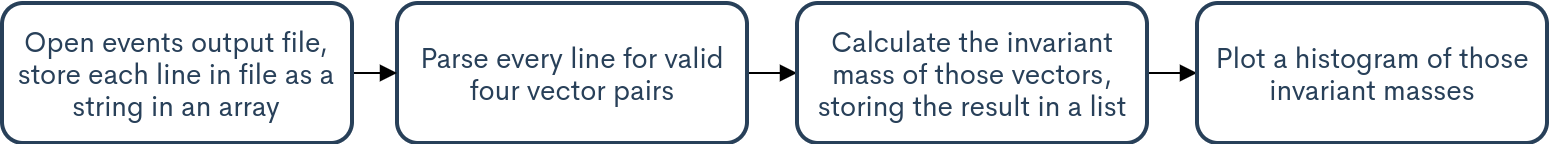
\includegraphics[scale=0.3]{diag.png}
\section*{Packages Required}
\begin{itemize}
  \item Numpy:      Powerful scientific computing package
  \item Matplotlib: Visual wrapper and renderer for Numpy
\end{itemize}
\section*{Functions or Structures Provided}
\begin{itemize}
  \item \texttt{function\_name(input type: input\_name)}:
    \textbf{description}
  \item \texttt{str\_to\_vec(string: line)}:
    \textbf{When parsing the lines contained in the output file,
    if the line contains data that is recognizable, converts the 
    relevent line from a human readable string, to a float array}
  \item \texttt{calc\_mass(float array: vec)}:
    \textbf{Given a four\_vec (float array) returns: }
    $\sqrt{E^2 + \vec{p}^2}$
  \item \texttt{calc\_mom(float array: vec)}:
    \textbf{Given a four\_vec (float array), returns the magnitude 
    of the momentum: } $\sqrt{\Sigma_ip_i^2}$
  \item \texttt{str\_starts\_as\_num(string: s)}:
    \textbf{Given a string (a line string in this case), checks if
    the string contains recognizable words in the lanugage of our
    computations. A word in this language is any postive or negative 
    array of numbers}
\end{itemize}
\end{document}
